\structure{ОСНОВНАЯ~ЧАСТЬ}

\section{Модель распределенной системы}

Эта часть задает основу для последующего анализа алгоритмов консенсуса, определяя
термины распределенной системы и консенсуса. Она задает условия и ограничения,
в которых эти алгоритмы могут быть применены.

\subsection{Определение распределенной системы}

Формального определения распределенной вычислительной системы в настоящее время
не существует. Из множества различных определений, можно выделить ироничное
определение Лесли Лампорта \cite{lamport_email}, которое он дал в мае 1987 года,
в своем письме коллегам по поводу очередного отключения электроэнергии в машинном
зале:

«Распределенной вычислительной системой можно назвать такую систему, в которой
отказ компьютера, о существовании которого вы даже не подозревали, может сделать
ваш собственный компьютер непригодным к использованию».

Эндрю Таненбаум предложил следующее определение \cite{tanenbaum_distributed_systems}:

«Распределенная вычислительная система (РВС) – это набор соединенных каналами
связи независимых компьютеров, которые с точки зрения пользователя некоторого
программного обеспечения выглядят единым целым».

Именно это определение и будет использоваться в данной работе. Таким образом,
в РВС есть несколько автономных участников (иногда называемых процессами, узлами
или репликами). Каждый участник обладает своим локальным состоянием. Участники
выполняют некий алгоритм, общаются, обмениваясь сообщениями через каналы связи
между ними. Вне системы существуют пользователи, которые могут отправлять запросы
к различным узлам системы и ожидать от них ответов.

\subsection{Модель каналов связи}

Связь через каналы часто ненадежна: сообщения могут теряться, задерживаться или
приходить в неправильном порядке. В качестве отправной точки взят канал с
приемлемыми потерями (fair-loss) \cite{cachin11}:

\begin{itemize}
    \item Допустимые потери. Если отправитель и получатель функционируют корректно и
        процесс отправляет сообщение бесконечно много раз, оно в конечном итоге
        будет доставлено бесконечное число раз.
    \item Ограниченное дублирование. Одно отправленное сообщение не будет доставлено
        бесконечное количество раз.
    \item Без создания. Канал не создает новых сообщений, то есть доставляются
        только те сообщения, которые были отправлены.
\end{itemize}

Канал с приемлемыми потерями является полезной абстракцией и первым строительным
блоком для протоколов обмена данными с сильными гарантиями. По своей сути он похож
на протокол UDP, который позволяет отправлять сообщения от одного процесса другому,
но не предлагает надежной семантики доставки на уровне протокола. Однако гарантии,
предоставляемые такой моделью недостаточны для построения надежных распределенных
систем.

Для повышения надежности связи можно использовать подтверждения (acknowledgement,
ACK), позволяющие получателю уведомить отправителя о доставке сообщения. Для
этого применяются полнодуплексные каналы связи и добавляются механизмы,
которые помогают различать сообщения, например, уникальные порядковые номера
(sequence numbers), монотонно возрастающие идентификаторы.

До тех пор, пока отправитель не получит подтверждение о доставке сообщения,
он не может быть уверен, было ли оно обработано, будет ли обработано в будущем,
утеряно, либо удаленный процесс вышел из строя до его получения. Отправитель
может повторно передать сообщение, но это может вызвать его дублирование.
Безопасная обработка дубликатов возможна только в случае, если выполняемая
операция является идемпотентной. Поскольку в реальных условиях не всегда удается
обеспечить идемпотентность операций, требуется применять эквивалентные гарантии.
Для этого можно использовать методы дедупликации (deduplication), предотвращающие
повторную обработку одного и того же сообщения.

Повторные передачи и несоблюдение порядка доставки могут приводить к неверному
порядку поступления сообщений. Благодаря введению порядковых номеров получатель
может использовать их для восстановления порядка и обеспечения обработки сообщений
по принципу FIFO (first-in, first-out).

Применив все описанные выше ограничения к каналу с приемлемыми ограничениями,
получаем совершенный канал (perfect link), предоставляющий гарантии \cite{cachin11}:

\begin{itemize}
    \item Надежная доставка. Каждое сообщение, отправленное один раз корректным
        процессом А корректному процессу Б, в конце концов будет доставлено.
    \item Порядок сообщений. Сообщения будут доставлены в том порядке, в котором
        они были отправлены.
    \item Без дублирования. Ни одно сообщение не будет обработано более одного раза.
    \item Без создания. Канал доставляет только отправленные сообщения, не создавая
        новые.
\end{itemize}

Именно совершенный канал будет использоваться как модель канала для построения
алгоритмов коненсуса распределенных систем. Он похож на протокол TCP.

Однако даже совершенный канал не защищает алгоритм от ситуации разделения сети,
под которой понимается, что два или более процесса не могут связаться друг
с другом. Независимые группы процессов могут продолжать выполнение алгоритмов
и выдывать противоречивые результаты, могут происходить асимметричые отказы
каналов, при которых сообщения могут проходить только в одну сторону, но не
обратно. Все это необхоимо учитывать при разработке алгоритмов в распределенных
системах.

\subsection{Определение консенсуса}

Алгоритм консенсуса описывает работу распределенной системы, которая при наличии
нескольких процессов, начинающих работу с некого начального состояния, переводит
все процессы в одинаковое состояние. Чтобы алгоритм консенсуса был корректным,
должны выполняться следующие условия \cite{petrov}:

\begin{itemize}
    \item Согласованность. Принимаемое протоколом решение должно быть единодушным:
        каждый процесс  выбирает некоторое значение, которое должно быть
        одинаковым для всех процессов.
    \item Действительность. Согласованное значение должно быть предложено одним
        из процессов. Т.е. это не может быть некое произвольное значение.
    \item Окончательность. Согласованность принимает окончательный характер после
        того, как уже не остается процессов, не достигших состояния принятия решения.
\end{itemize}

\subsection{Теорема Фишера-Линча-Патерсона}

Мысленный эксперимент, известный как «задача двух генералов», наглядно
иллюстрирует сложности обеспечения консенсуса в распределенных системах.
Эксперимент демонстрирует, что в асинхронной системе, где нет временных
ограничений на доставку и ответы, невозможно достичь полного согласия между
сторонами, даже с использованием многочисленных подтверждений.

Суть задачи такова: две армии под командованием генералов расположены по разные
стороны от города и должны атаковать одновременно, чтобы достичь успеха.
Генералы передают сообщения через посланников, чтобы договориться об атаке.
Однако посланники могут быть перехвачены или не доставить сообщение, что
создает неопределенность. То есть генералам необходимо достичь консенсуса
по времени начала атаки.

Например, генерал А отправляет сообщение MSG(N), предлагая атаку в определенное
время. Генерал Б, получив сообщение, посылает подтверждение ACK(MSG(N)). На
рис. \ref{fig:generals} показано, что сообщение отправляется в одну сторону и
подтверждается  другой стороной.

\begin{figure}
  \centering
  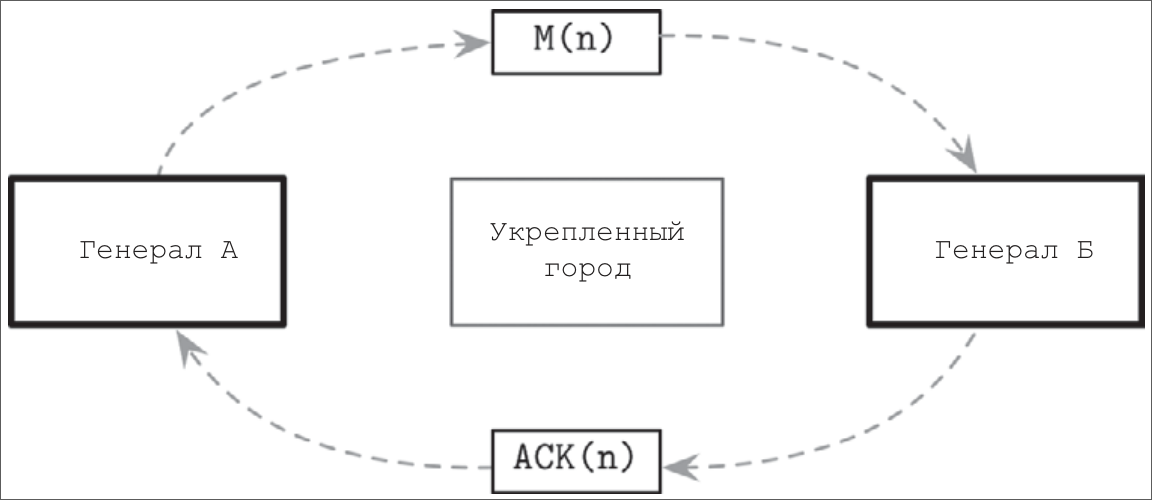
\includegraphics[scale=0.4]{inc/generals.png}
  \caption{Задача двух генералов}
  \label{fig:generals}
\end{figure}

Однако генерал А не может быть уверен, что это подтверждение дошло, оно может
быть утеряно. Чтобы устранить сомнения, требуется второе подтверждение —
ACK(ACK(MSG(N))). Этот процесс может продолжаться бесконечно, поскольку всегда
остается риск того, что последнее сообщение не достигло адресата.

В задаче не сделано предположений о времени, не установлено лимита, за которое
генералы должны ответить, связь полностью асинхронна.

В работе Фишера, Линча и Патерсона рассматривается проблема, известная как
невозможность ФЛП (FLP Impossibility) \cite{fischer85}. Эта теорема, также
именуемая теоремой Фишера–Линча–Патерсона, изучает консенсус в системах, где
процессы начинают с начального значения и стремятся согласовать новое общее
значение. После выполнения алгоритма это значение должно быть одинаковым для
всех корректно работающих процессов.

В исследовании предполагается полностью асинхронная среда, где процессы не
имеют общего времени. Алгоритмы в таких системах не могут полагаться
на время ожидания, а у процесса отсутствует возможность определить, отказал ли
другой процесс или просто работает медленно. В статье доказывается, что при
указанных предположениях невозможно создать протокол, который гарантирует
достижение консенсуса за ограниченное время. Даже один сбой процесса, не
сопровождающийся уведомлением, делает консенсус недостижимым для полностью
асинхронной распределенной системы.

Тем не менее, теорема ФЛП не утверждает, что достижение консенсуса в принципе
невозможно. Она лишь показывает, что в асинхронной системе консенсус не всегда
достижим за конечное время. В реальных системах часто присутствует некоторая
степень синхронности, и эту особенность нужно учитывать.

\subsection{Синхронность}

Из теоремы ФЛП следует, что ключевой характеристикой распределенной системы
является предположение о времени. В асинхронных системах невозможно
гарантировать ограниченные задержки в доставке сообщений, упорядоченность их
получения. Процесс выдает ответ через неопределенной долгое время.

Однако, одним из аргументов против асинхронных систем является их оторванность
от реальности: процессы не имеют произвольно разные скорости обработки, а
задержки передачи сообщений не бывают бесконечными.

Можно сделать предположения менее строгими, считая систему синхронной. Может
предполагаться, что процессы работают с сопоставимыми скоростями, задержки
передачи сообщений в канале ограничены, их доставка не может занимать
бесконечно долгое время.

В модель синхронной системы также можно добавить локальные для процесса
синхронизированные часы: при этом существует некоторая верхняя граница в раз­
нице во времени между двумя локальными для процессов источниками времени
\cite{cachin11}.

Свойства асинхронных и синхронных моделей можно объединить, рассматривая
систему как частично синхронную. Частично синхронная система обладает некото­
рыми свойствами синхронной системы, но при этом ограничения на время доставки
сообщений, уход показаний часов и относительные скорости обработки могут быть
приблизительными и действовать лишь в большинстве случаев.

\subsection{Модели отказов}

Модель отказов описывает, каким образом могут происходить сбои в работе
процессов распределенной системы. Например, можно предположить, что процесс
может полностью завершить работу и не восстановиться, восстановиться через
некоторое время или начать выдавать некорректные данные из-за сбоя или
преднамеренно.

Поскольку процессы в распределенных системах взаимодействуют друг с другом
при выполнении алгоритма, сбои в одном из них могут нарушить выполнение всей
системы. Для разработки алгоритмов в распределенных системах необходимо понимать,
какие отказы могут случиться, чтобы правильно обрабатывать каждый из них.

\subsubsection*{Аварийное завершение}

В этой модели предполагается, что процесс перестает выполнять шаги алгоритма
и не отправляет сообщений другим процессам. После сбоя процесс остается в этом
состоянии и больше не участвует в текущем выполнении алгоритма.

Важно отметить, что эта модель не запрещает восстановление процессов. Процесс
может восстановиться, синхронизироваться с текущим состоянием системы и
участвовать в новых раундах алгоритма.

Процесс, который восстанавливается после сбоя, может продолжить выполнение с
последнего известного ему шага. Алгоритмы, поддерживающие восстановление,
должны вводить в систему понятия устойчивого состояния алгоритма и протокола
восстановления \cite{skeen83}.

\subsubsection*{Пропуск}

В этой модели процесс пропускает выполнение отдельных шагов алгоритма, либо
эти шаги невидимы для других участников, либо процесс не может отправлять и
получать сообщения. Пропуски включают сетевые сбои, вызванные неисправностями
каналов связи, отказами оборудования или перегрузкой сети.

Пропуски возникают, когда алгоритм не завершает определенные действия, или их
результаты не достигают других процессов. Например, потерянное сообщение может
привести к тому, что отправитель считает его доставленным, несмотря на его
окончательную утрату.

\subsubsection*{Византийские ошибки}

Произвольные, или византийские, ошибки (Byzantine faults) представляют собой
наиболее сложный класс отказов. В этом случае процесс продолжает выполнять шаги
алгоритма, но делает это некорректно.

Такие сбои могут быть вызваны ошибками в программном обеспечении, выполнением
разных версий алгоритма или намеренными действиями злоумышленников. Например,
в распределенных системах без централизованного управления, таких как
криптовалюты, процессы могут фальсифицировать данные, чтобы ввести систему в
заблуждение.

\subsubsection*{Обработка отказов}

Одним из способом обработки отказов при невизантийских ошибках является введение
в алгоритм избыточности. Таким образом отказ может быть замаскирован: даже если
один или несколько процессов откажут, то пользователь этого не заметит
\cite{christian91}. Raft и Paxos, которые будут рассмотрены в данной работе,
основываются на модели отказов и минимизирует влияение отказов путем
использования избыточности процессов.

В случае работы в распределенной системе с византийскими ошибками используется
перекрестная проверка других узлов на каждом шаге, поскольку узлы не могут
полагаться друг на друга или на лидера и должны проверять поведение других узлов,
сравнивая возвращаемые результаты с ответами большинства. PBFT, PoW, PoS борются
с ошибками именно так.

\subsection{Итоги}

Таким образом, к распределенной системе, в которой будет исполняться любой из
описанных в данной работе алгоритм консенсуса, применяются следующие ограничения:

\begin{itemize}
    \item Система передает сообщения по совершенным каналам, однако допустимо
        разделение сети.
    \item Необходимо учитывать возможность отказа узлов: аварийное завершение и
        пропуск части алгоритма процессом.
    \item В системе невозможны византийские ошибки. Предполагается, что все узлы
        честные и выполняют свои функции корректно.
    \item Система является частично синхронной, в ней существует понятие времени,
        которое используется для синхронизации локальных часов. Сообщения в системе
        могут отправляться бесконечно, процессы могут работать с произвольной
        скоростью.
\end{itemize}
